\documentclass[twoside]{report}

\newcommand{\RootPath}{../../../}
\newcommand{\MyPath}{\RootPath Boostan/tex/}

\usepackage{adjustbox}
\usepackage{ptext}
\usepackage{algorithm}
\usepackage{algorithmic}

\input{\MyPath Boostan-Thesis}

%واژه‌های خود را در فایل words وارد کنید، و در ضمن اختصارات را نیز در abbre وارد کنید. 
\newword{Architecture}{Architecture}{معماری}{معماری‌ها}
\newword{Average}{Average}{میانگین}{}
\newword{Call}{Call}{تماس}{تماس‌ها}
\newword{CloudComputing}{Cloud Computing}{رایانش ابری‌}{‌}
\newword{Delay}{Delay}{تاخیر}{تاخیرها}
\newword{DriveTest}{Drive Test}{درایو تست}{}
\newword{GaussianDistribution}{Gaussian Distribution}{توزیع گاوسی}{توزیع‌های گاوسی}
\newword{PacketSwitching}{Packet Switching}{کلیدزنی بسته‌ای}{}
\newword{PacketSwitch}{Packet Switch}{کلیدزنی بسته‌ای}{}
\newword{PenetrationCoefficient}{Penetration Coefficient}{ضریب نفوذ}{ضرایب نفوذ}
\newword{PropagationChannelModel}{Propagation Channel Model}{مدل انتشار کانال}{مدل‌های انتشار کانال}
\newword{QualityofExperience}{Quality of Experience}{کیفیت تجربه}{کیفیت تجربه}
\newword{QualityofService}{Quality of Service}{کیفیت خدمت}{کیفیت خدمات}
\newword{RandomVariable}{Random Variable}{متغیر تصادفی}{متغیرهای تصادفی}
\newword{StandardDeviation}{Standard Deviation}{انحراف استاندارد}{}

\newacronym{ACK}{ACK}{Acknowledgement}

\newacronym{ACI}{ACI}{Application Control Interface}

\newacronym{ACIR}{ACIR}{Adjacent Channel Interference Ratio}

\newacronym{ACLC}{ACLC}{Adaptive Configuration of Logical Channels}

\newacronym{ACLP}{ACLP}{Adjacent Channel Leakage Power}

\title{موضوع پایان‌نامه را در این قسمت بنویسید}
\faculity{نام دانشکده}
\group{نام گروه}
\author{نام نویسنده}
\forwhat{پایان‌نامه کارشناسی ارشد}
\field{در رشته‌ ........}
\logofile{Logo/Fa}
\logoScale{0.25\linewidth}
\supervisor{دکتر .....}
\date{شهریور 1403}

\graphicspath{{./Pic/}}

\begin{document}
\pagenumbering{gobble}
\thesisStyleO
\newpage
\Godpage
\newpage
\clearpage\newpage
\begin{table}
\begin{tabular}{ccc}

\includegraphics[width=.15\textwidth]{Pic/logo}&
\begin{minipage}{0.55\linewidth}
\vskip 0.9cm
\begin{center}\Large
\typefontR{\Large
دانشگاه تهران 
}
 \\* [0.5cm]
پرديس دانشکده های فنی\\ [0.5cm]
\end{center}
\end{minipage}
&
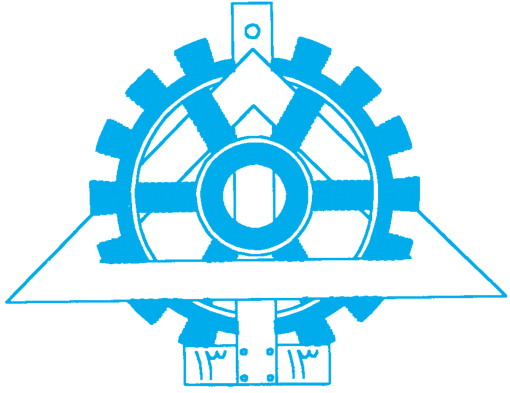
\includegraphics[width=.15\textwidth]{Pic/logo2}
\end{tabular}
\end{table}
\begin{center}
\vskip 1.5cm
رساله برای دریافت درجه‌ی دکتری تخصصی در رشته مهندسی  کامپیوتر گرایش نرم‌افزار

\vskip 5pt \textbf{عنوان:}
بررسی و ارزیابی حفظ حریم‌زمانی در شبکه‌های ارتباطی با استفاده از تئوری صف

\vskip 5pt \textbf{نگارش:} 
ابوالفضل دیانت

\end{center}
\vskip 0.9cm\indent
این پایان‌نامه در تاریخ 1395/11/20 در مقابل هیات داوران دفاع گردید و مورد تصویب قرار گرفت. 
\vskip 0.9cm
\vskip 5pt \textbf{
رییس دانشکده‌ی مهندسی برق و کامپیوتر:} دکتر مجید نیلی احمدآبادی

\vskip 5pt \textbf{
معاون پژوهشی و تحصیلات تکمیلی دانشکده مهندسی برق و کامپیوتر:} دکتر بابک نجار اعرابی

\vskip 5pt \textbf{
استاد راهنما:} دکتر احمد خونساری

\vskip 5pt \textbf{
عضو هیات داوران:} دکتر بابک خلج

\vskip 5pt \textbf{
عضو هیات داوران:} دکتر فرید آشتیانی

\vskip 5pt \textbf{
عضو هیات داوران:} دکتر مهدی کارگهی

\vskip 5pt \textbf{
عضو هیات داوران:} دکتر بهنام بهرک

%\vskip 5pt \textbf{
%عضو هیات داوران:} دکتر .... 





















\clearpage\newpage
\makeatletter

\begin{center}
{\LARGE{\textbf{تأییدیه صحت و اصالت نتایج}}}\\*[1cm]
باسمه تعالی
\end{center}


این‌جانب
\textbf{\@author}
به شماره دانشجویی
\textbf{\@authorCode}
دانشجو رشته \textbf{مهندسی کامپیوتر} گرایش \textbf{شبکه‌های کامپیوتری} مقطع تحصیلی \textbf{کارشناسی ارشد }تایید می‌نمایم که کلیه مندرجات در این پایان‌نامه حاصل کار پژوهشی اینجانب تحت نظارت و راهنمایی عضو هیأت علمی دانشگاه علم و صنعت ایران، بدون هرگونه دخل و تصرف انجام گرفته و موارد نسخه‌برداری شده از آثار دیگران، مطابق مقررات و ضوابط ارجاع داده شده و ویژگی‌های کامل منابع را در فهرست منابع ذکر کرده‌ام. این پایان‌نامه پیش‌تر برای احراز هیچ مدرکی ارائه نگردیده است. 

در صورت اثبات خلاف مندرجات فوق، به تشخیص دانشگاه مطابق با ضوابط و مقررات حاکم (قانون حمایت از حقوق مولفان و منصفان و قانون ترجمه، تکثیر و نشریات و آثار صوتی، ضوابط و مقررات آموزشی و پژوهشی، انضباطی و غیره) با اینجانب رفتار خواهد شد و حق هرگونه اعتراض در خصوص احقاق حقوق مکتسب و تشخیص و تعیین تخلف و مجازات را از خویش سلب می‌نمایم. در ضمن، مسئولیت هرگونه پاسخگویی به اشخاص اعم از حقیقی و حقوقی و مراجع ذی‌صلاح (اعم از اداری و قضایی) به عهده اینجانب خواهد بود و دانشگاه هیچ گونه مسئولیتی در این خصوص نخواهد داشت. 

کلیه نتایج و حقوق حاصل از این پایان‌نامه متعلق به دانشگاه علم و صنعت ایران است. هرگونه استفاده از نتایج علمی و عملی و واگذاری اطلاعات به دیگران یا چاپ و تکثیر، نسخه‌برداری، ترجمه و اقتباس از این پایان‌نامه بدون موافقت کتبی دانشگاه علم و صنعت ایران ممنوع است. نقل مطالب با ذکر منبع بلامانع است. 


\vskip 1cm
\begin{flushleft}
\begin{table}[H]
\raggedright
\begin{tabular}{rr}
نام و نام‌خانوادگی دانشجو: &
\@author \\*[5mm]
تاریخ: &
\@date \\*[5mm]
امضای دانشجو: &
\\
\end{tabular}
\end{table}
\end{flushleft}
\makeatother

\newpage
\vspace{4cm}

{\nastaliq
	{\Huge
		تقدیم به همه آنهایی که 
		\vspace{1.5cm}
		
		\hspace{3cm}
		می خواهند بیشتر بدانند
}}


\newpage
{\nastaliq\LARGE
سپاس‌گزاری...
}
\\[2cm]
 ماحصل آموخته هایم را تقدیم می‌کنم به آنان که مهر آسمانی‌شان آرام بخش آلام زمینی ام است.
 
به استوارترین تکیه گاهم،دستان پرمهر پدرم...

به سبزترین نگاه زندگیم،چشمان سبز مادرم...

که هرچه آموختم در مکتب عشق شما آموختم و هرچه بکوشم قطره ای از دریای بی کران مهربانی‌تان را سپاس نتوانم بگویم.

امروز هستی ام به امید شماست و فردا کلید باغ بهشتم رضای شما...

ره‌آوردی گران سنگ تر از این ارزان نداشتم تا به خاک پایتان نثار کنم؛ باشد که حاصل تلاشم نسیم گونه غبار خستگی‌تان را بزداید. بوسه بر دستان پرمهرتان.

هم‌چنین بر خود واجب می‌دانم از زحمات استاد راهنمای خود، جناب آقای دکتر ..... صمیمانه تشکر و  قدردانی کنم  که قطعاً بدون راهنمایی‌های‌ ایشان، این کار به انجام نمی‌رسید. 

\clearpage
\section*{چکیده}
در این قسمت چکیده پایان‌نامه را بنویسید.

\vskip 5mm
\noindent\textbf{کلمات کلیدی}:
کلمات کلیدی را در این قسمت وارد کنید. 

\clearpage
\pagenumbering{alph}
\tableofcontents
\listoffigures
\listoftables
\printabbreviation
\pagenumbering{arabic}

\pagestyle{mystyle}
\chapter{مقدمه}
\label{chap:intro}

\begin{figure}
\includegraphics[width=\linewidth]{/ETCMobile/0GTo6G/mainFig}
\caption{\lofimage{/ETCMobile/0GTo6G/mainFig}
نسل‌های مختلف شبکه‌های تلفن‌همراه
}
\label{fig:0GTo6G}
\end{figure}
امروزه شاهد گسترش روزافزون شبکه‌های تلفن‌همراه در سرتاسر جهان هستیم. اطلاعات آماری حکایت از آن دارد که تا انتهای سال ۲۰۲۳ از میان 
$8.02$
میلیارد انسانی که بر روی کره زمین زندگی می‌کنند، در حدود 
$5.6$
میلیارد نفر از شبکه‌های تلفن‌همراه استفاده می‌کنند که این خود حاکی از
\gls{PenetrationCoefficient} $69$
درصدی این شبکه‌ها است. برطبق گزارش مؤسسه
\gls{GSMA}،
فناوری تلفن‌همراه و خدمات مرتبط با آن در سال 2023، در حدود 
$5.7$
تریلیون دلار ($5.4\%$ تولید ناخالص داخلی) ارزش‌افزوده به همراه داشته
\cite{GSMA2024MobileEconomy}.
این حجم شگرف چرخش مالی، منجر به ایجاد فرصت‌های پژوهشی، صنعتی و تجاری بسیاری گشته است. اهمیت شبکه‌های تلفن‌همراه، زمانی آشکار می‌گردد که بدانیم رشد و توسعه این شبکه‌ها، مرهون توسعه فناوری‌‌هایی نظیر 
\gls{MIMO}، \gls{IOT}، \gls{SDN}، \gls{NFV}و \gls{CloudComputing}
بوده است. این مهم به‌ویژه در شبکه‌های نسل پنج، بیش‌ازپیش خودنمایی می‌کند. 

شروع توسعه شبکه‌های نسل دو به‌مانند 
\gls{GSM}
در دهه 1980، با تمرکز بر ارائه خدماتی نظیر تبادل
\gls{Call} صوتی و \gls{SMS}
شکل گرفت. اما به‌مرور نقطه تمرکز به ارائه خدمات مبتنی بر 
\gls{PacketSwitch}
نیز معطوف گشت
(\gls{GPRS} و \lr{Edge}).
توسعه شبکه‌های نسل سه
\gls{UMTS}،
بسان پلی بود که ما را بیش‌ازپیش، بدین هدف نزدیک‌تر می‌نمود. در سال 2004، ایده‌های اولیه شبکه‌های نسل چهار 
(\gls{LTE} و \lr{LTE-Adv})،
با هدف ایجاد یک شبکه دسترسی با سرعت و ظرفیت بالا، قابلیت ارائه خدمات مختلف و انعطاف در تعامل با دیگر شبکه‌ها، تدوین گشت. در حال حاضر 
\lr{4G}
با سرعت سرسام‌آوری در حال توسعه جایگاه خویش در میان شبکه‌های تلفن همراه است، تا جایی که در سال 2018 در حدود 47 درصد کل ارتباطات تلفن همراه را به خود تخصیص داده است
\cite{globenewswire2019}. 




\gls{ITU} 
در پروژه‎ 
\lr{IMT-2020}، 
سه ویژگی کلیدی 
\lr{5G} 
را ارتباطات پرشمار ماشینی (مانند 
\lr{IoT})، 
پایدار و با 
\gls{Delay} 
اندک بر می‌شمارد. انتظار بر آن است که 
\lr{5G} 
از لحاظ پوشش، سرعت و تأخیر عملکرد چشمگیرتری نسبت به 
\lr{4G} 
از خود نشان دهد. برطبق نمودار 
\lr{Gartner} 
سرمایه‌گذاری و کار بر روی 
\lr{5G} 
حداقل تا یک دهه آینده ادامه خواهد داشت. تحقیقات بر روی شبکه‌های نسل جدید 
\lr{6G} 
از هم اکنون آغاز گشته و رد پای آن را در برخی از مقالات پژوهشی موجود در این حوزه می‌توان یافت 
(\autoref{fig:0GTo6G}).



\section{طرح مسئله}
هنگامی که کنوث پیش‌نمایش جلد دوم کتاب خود را
(\lr{The Art of Computer Programming})
در ۳۰ مارس ۱۹۷۷ دریافت کرد، متوجه شد که بسیار بدشکل است. در همین زمان بود که او کتاب
\lr{Artificial Intelligence}
نوشته
\lr{Patrick Winston}
که با حروف‌چینی دیجیتالی تهیه شده بود، را مشاهده نمود، و به این نوع از حروف‌چینی علاقه‌مند شد. پیش‌نمایش‌های مأیوس‌کننده در نهایت موجب شدند که او تصمیم بگیرد با طراحی سیستم حروف‌چینی خود برمبنای حروف‌چینی دیجیتالی، این مشکل را یک بار و برای همیشه حل کند. کنوث دریافت که معنای حروف‌چینی دیجیتالی این است که بتوان یک چیدمان درست از صفرها و یک‌ها (نقاط سفید و سیاه) را در کنار یکدیگر قرار داد. یافتن قواعد درست و زیبا برای نگارش متون ریاضی و تبدیل آن به چیدمان صحیحی از صفرها ویک‌ها، کاری بود که کنوث فکر می‌کرد آن‌را می‌تواند در ظرف شش ماه تا تعطيلات دانشگاهي سال ۱۹۷۸ به پایان برساند، اما آن‌چه که اتفاق افتاد این بود که در نهایت در ۱۹۸۹، یعنی ده سال بعد، این کار به اتمام رسید، و بدین‌سان 
\lr{\TeX{}}
متولد شد .... 

\lr{\TeX{}}
یک زبان نشانه‌گذاری
(\lr{Markup Language})
است.  محتوا در یک پروندهٔ متنی نوشته می‌شود و نشانه‌گذاری‌ها به شکل فرمان‌هایی بین متن قرارمی‌گیرند و مشخص می‌کنند که هر بخش از نوشته چه‌طور نمایش یابد. مفسر لاتک آن پرونده را می‌خواند، محتوا را به شکل یک نوشته درمی‌آورد و یک پروندهٔ خروجی می‌سازد. 
\begin{lstlisting}[language=TeX, numbers=none]
% Plain TeX for a 1 page document
\TeX{} is good at typesetting words like `fjord', `efficiency',
and `fiasco'. It is also good at typesetting math like,
$a^2 + b^2 = c^2$.
\beginsection 1. Introduction.
This is an example.
\bye
\end{lstlisting}
دقیقا برعکس نرم‌افزارهای واژه‌پرداز معمولی مثال 
\lr{Microsoft Word}
که بر اساس
\begin{center}
\lr{WYSIWYG (\textcolor{Plum}{\textit{What you see is what you get}})}
\end{center}
کار می‌کنند .... کنوث به کسانی که در 
\lr{\TeX{}}
 اشکالی بیابند و آن را گزارش کنند، جایزهٔ نقدی می‌دهد. جایزهٔ هر اشکال از 
$2.56$
 دلار آغاز شده و هر سال دو برابر شده‌است. این باعث فقر کنوث نشده‌است، چرا که تعداد بسیار کمی باگ گزارش شده‌است. علاوه بر این، افراد معمولاً به جای نقد کردن چک، آن را قاب می‌گیرند تا ثابت کنند در 
\lr{\TeX{}}
 اشکالی یافته‌اند.

\lr{\TeX{}}
یک زبان برنامه‌نویسی واقعی، گسترده و برای کاربر عادی بسیار مشکل است 
\lr{\LaTeX}
یک سامانه‌ی آماده‌سازی و حروف‌چینی نوشتار بر پایه
\lr{\TeX{}}
است، که از آن به عنوان موتور حروف‌چینی استفاده می‌کند.  در واقع هر دستور \lr{\LaTeX}، از مجموعه‌ای پیچیده از دستورات \lr{\TeX{}} تشکیل شده است، که گردابه‌ای بزرگ از صورت‌های توسعه‌یافته‌ی \lr{\TeX{}} را تشکیل می‌دهد. بدین‌سان خانواده 
\lr{\TeX{}}
روزبه‌روز گسترش یافت:
\lr{Xe\TeX{}}, \lr{Pdf\TeX{}}, \lr{Lua\TeX{}} و ... .

چرا باید از \LaTeX استفاده کنیم؟ به هزاران دلیل .....
\begin{itemize}
\tick \textcolor{Plum}{\textbf{جدابودن محتوا و ظاهر نوشته‌}}:
برتری بزرگ \lr{\LaTeX} در این موضوع برای کاربران \lr{Word} چندان واضح نیست، زیرا آن‌ها نمی‌دانند که این ویژگی چه‌قدر خوب است. وقتی با 
\lr{\LaTeX}
 نوشتهٔ خود را می‌نویسید، فقط به محتوای نوشته فکر می‌کنید و ساختار متن را مستقیماً به \lr{\LaTeX} می‌گویید ... 
\tick \textcolor{Plum}{\textbf{کیفیت}}:
به سختی می‌توان این موضوع را انکار کرد که کیفیت خروجی‌های لاتک بسیار فراتر از خروجی‌های
\lr{Word}
است.
\tick \textcolor{Plum}{\textbf{تسلط بر نوشته}}:
حتی در نوشته‌های کوتاه هم شاید شما با رفتار غیرهوشمندانهٔ \lr{Word} روبه‌رو شده‌باشید. مثلاً در یک نوشتهٔ ۳۰ صفحه‌ای پر از شکل و جدول، یک بعدازظهر را صرف می‌کنید تا همه‌چیز مرتب شود؛
\tick \textcolor{Plum}{\textbf{استانداردنویسی}}:
\lr{\LaTeX}
به شدت تلاش می‌کند تا شما را مجبور کند تا استاندارد بنویسید ... 
\tick \textcolor{Plum}{\textbf{رایگان}}:
در این مورد لاتک هیچ حرفی باقی نمی‌گذارد، چون رایگان است! ضرب‌المثل «هر چی بیشتر پول بدی، بیشتر آش می‌خوری» دربارهٔ لاتک صادق نیست.
\tick \textcolor{Plum}{\textbf{انعطاف‌پذیری}}:
می‌توانید با لاتک هرکاری که فکرش را می‌کنید انجام دهید! در طول سالیان دراز، بسته‌های بسیار زیادی ساخته شده‌اند که ویژگی‌های لاتک را گسترش می‌دهند. برای نمونه، بسته
\lr{Bibtex}, \lr{glossaries}, \lr{listings}, \lr{tikz} و .... .
\tick \textcolor{Plum}{\textbf{پایداری‌}}: \lr{Word} 
در هنگام ویرایش نوشته‌های طولانی زیاد قفل می‌کند، اما 
\lr{\TeX{}} .... . 
\tick \textcolor{Plum}{\textbf{امنیت‌}}:
 در لاتک نیازی نیست نگران ویروس‌هایی باشید که در ماکروهای \lr{Word} پنهان می‌شوند!
\tick \textcolor{Plum}{\textbf{مستقل از سیستم‌عامل}}
\tick \textcolor{Plum}{\textbf{انجمن‌های پرسش و پاسخ بسیار قوی}}
\end{itemize}

برای من این تغییر کاملاً سودآور بود، زیرا الان می‌توانم نوشته‌ها و گزارش‌هایم را با سرعت بیشتری بنویسم. هرکسی می‌تواند لاتک را امتحان کند و تفاوتش را ببیند و تصمیم بگیرد. اما هر کس که وارد دنیای
\lr{\LaTeX}
در آن غرق شد ... 

\begin{figure}
\includegraphics[width=0.9\linewidth]{/calcdistance/mainFig}
\caption{\lofimage{/calcdistance/mainFig}%
نمونه شکل ساخته شده با 
\lr{Tikz}}
\label{fig:cellgeom}
\end{figure}

\section{چالش‌ها و انگیزه}

\section{نوآوری‌ها}
نوآوری‌های این پایان‌نامه به طور خلاصه به شرح زیر است:
 \begin{itemize} 
 \tick 
ارایه یک روش نوین برای بهینه‌سازی ....
 \end{itemize}
 

\section{ساختار گزارش}
نخست در
\autoref{chap:concepts}،
تعاریف و مفاهیم مبنایی در حوزه‌ی شبکه‌های تلفن همراه مانند معماری 
\gls{UE}
بیان می‌شود. در
\autoref{chap:relatedworks}،
به معرفی و بررسی کارهای پیشین انجام شده در این حوزه پرداخته خواهد شد. در 
\autoref{chap:approach}،
روش پیشنهادی این پژوهش ارائه خواهد شد که شامل استفاده از داده‌های جمع‌آوری‌شده از \gls{DriveTest}، مدل‌سازی کانال، و به‌کارگیری روش‌های هوش مصنوعی برای پیش‌بینی دقیق‌تر و بهبود عملکرد شبکه است. در 
\autoref{chap:simulation}
نتایج به‌دست‌آمده از آزمایش‌های متعدد روش پیشنهادی را تحلیل کرده و در نهایت در
\autoref{chap:conclusion}
به جمع‌بندی این پژوهش خواهیم پرداخت.

\chapter{مفاهیم پایه‌ای}
\label{chap:concepts}
در ابتدای هر فصل از پایان‌نامه، سعی کنید نخست بدون شروع هرگونه 
\lr{Section}، 
به طور خلاصه بگویید که قرار است در این فصل در مورد چه چیزی صحبت کنید. به عنوان مثال در این فصل، نخست در 
\autoref{sec:boostanenv}،
در مورد محیط‌های مختلفی که می‌توانید در استایل بوستان از آن استفاده کنید، صحبت خواهیم کرد. سپس در 
\autoref{sec:codeintext}،
در مورد نحوه وارد کردن یک کد در متن سخن به میان خواهد آمد. 

\section{محیط‌های مختلف در استایل بوستان}\index{محیط}
\label{sec:boostanenv}
‎\ptext[1]
\subsection{محیط نکات}
\begin{note}
شهر مردگان، شهر انسان های «بی دفاع» است. این تعبیر اقتباس از قرآن کریم است که «غیبت» را خوردن گوشت «مرده» خوانده است. 
\begin{equation}
A = B + \sin (x)
\end{equation}
در تفاسیر آمده است که خداوند «انسان بی دفاع» را که به دلیل عدم حضور در مجلس بدگویی نمی تواند از خود دفاع کند، «مرده» دانسته است. پس آنجا که نسبت های ناروا دادن مباح، و دفاع کردن ممنوع است، در حقیقت «شهر مردگان» است.
\end{note}
‎\ptext[2]
\begin{problem}
شهر مردگان، شهر انسان های «بی دفاع» است. این تعبیر اقتباس از قرآن کریم است که «غیبت» را خوردن گوشت «مرده» خوانده است . در تفاسیر آمده است که خداوند «انسان بی دفاع» را که به دلیل عدم حضور در مجلس بدگویی نمی تواند از خود دفاع کند، «مرده» دانسته است. پس آنجا که نسبت های ناروا دادن مباح، و دفاع کردن ممنوع است، در حقیقت «شهر مردگان» است.


\end{problem}
‎\ptext[3]
\begin{refer}
شهر مردگان، شهر انسان های «بی دفاع» است. این تعبیر اقتباس از قرآن کریم است که «غیبت» را خوردن گوشت «مرده» خوانده است.
\begin{latin}
\lstset{numbers=none,frame=none}
\begin{lstlisting}
for i:=maxint to 0 do
begin
{ do nothing }
end;
\end{lstlisting}
\end{latin}
  در تفاسیر آمده است که خداوند «انسان بی دفاع» را که به دلیل عدم حضور در مجلس بدگویی نمی تواند از خود دفاع کند، «مرده» دانسته است. پس آنجا که نسبت های ناروا دادن مباح، و دفاع کردن ممنوع است، در حقیقت «شهر مردگان» است.
\end{refer}

\begin{info}
شهر مردگان، شهر انسان های «بی دفاع» است. این تعبیر اقتباس از قرآن کریم است که «غیبت» را خوردن گوشت «مرده» خوانده است . 
در تفاسیر آمده است که خداوند «انسان بی دفاع» را که به دلیل عدم حضور در مجلس بدگویی نمی تواند از خود دفاع کند، «مرده» دانسته است. پس آنجا که نسبت های ناروا دادن مباح، و دفاع کردن ممنوع است، در حقیقت «شهر مردگان» است.
\begin{equation}
A = B + \sin (x)
\end{equation}
\end{info}

\index{نکته}
\begin{warning}{نکات مهم}
شهر مردگان، شهر انسان های «بی دفاع» است. این تعبیر اقتباس از قرآن کریم است که «غیبت» را خوردن گوشت «مرده» خوانده است . در تفاسیر آمده است که خداوند «انسان بی دفاع» را که به دلیل عدم حضور در مجلس بدگویی نمی تواند از خود دفاع کند، «مرده» دانسته است. پس آنجا که نسبت های ناروا دادن مباح، و دفاع کردن ممنوع است، در حقیقت «شهر مردگان» است.
\end{warning}


\begin{goal}{نکات مهم}
شهر مردگان، شهر انسان های «بی دفاع» است. این تعبیر اقتباس از قرآن کریم است که «غیبت» را خوردن گوشت «مرده» خوانده است . 

در تفاسیر آمده است که خداوند «انسان بی دفاع» را که به دلیل عدم حضور در مجلس بدگویی نمی تواند از خود دفاع کند، «مرده» دانسته است.

  پس آنجا که نسبت های ناروا دادن مباح، و دفاع کردن ممنوع است، در حقیقت «شهر مردگان» است.
\end{goal}

\subsection{محیط‌های ریاضی}
کارکرد لاتک مبتنی بر این اندیشه است که نویسندگان باید قادر باشند بر نوشتن در درون ساختار منطقی متن‌شان تمرکز کنند، نه اینکه وقت خود را برای کار کردن بر روی جزئیات شکل‌دهی صرف کنند. 
\begin{ntdefinition}
شهر مردگان، شهر انسان های «بی دفاع» است. 
\end{ntdefinition}
کارکرد لاتک مبتنی بر این اندیشه است که نویسندگان باید قادر باشند بر نوشتن در درون ساختار منطقی متن‌شان تمرکز کنند، نه اینکه وقت خود را برای کار کردن بر روی جزئیات شکل‌دهی صرف کنند. 
\begin{ntdefinition}
شهر مردگان، شهر انسان های «بی دفاع» است. 
\end{ntdefinition}
کارکرد لاتک مبتنی بر این اندیشه است که نویسندگان باید قادر باشند بر نوشتن در درون ساختار منطقی متن‌شان تمرکز کنند، نه اینکه وقت خود را برای کار کردن بر روی جزئیات شکل‌دهی صرف کنند. 
\begin{ntexample}
شهر مردگان، شهر انسان های «بی دفاع» است. 
\end{ntexample}
کارکرد لاتک مبتنی بر این اندیشه است که نویسندگان باید قادر باشند بر نوشتن در درون ساختار منطقی متن‌شان تمرکز کنند، نه اینکه وقت خود را برای کار کردن بر روی جزئیات شکل‌دهی صرف کنند. 
\begin{ntexample}
شهر مردگان، شهر انسان های «بی دفاع» است. 
\end{ntexample}
\begin{ntsolution}
شهر مردگان، شهر انسان های «بی دفاع» است. این تعبیر اقتباس از قرآن کریم است که «غیبت» را خوردن گوشت «مرده» خوانده است . در تفاسیر آمده است که خداوند «انسان بی دفاع» را که به دلیل عدم حضور در مجلس بدگویی نمی تواند از خود دفاع کند، «مرده» دانسته است. پس آنجا که نسبت های ناروا دادن مباح، و دفاع کردن ممنوع است، در حقیقت «شهر مردگان» است.
\end{ntsolution}
کارکرد لاتک مبتنی بر این اندیشه است که نویسندگان باید قادر باشند بر نوشتن در درون ساختار منطقی متن‌شان تمرکز کنند، نه اینکه وقت خود را برای کار کردن بر روی جزئیات شکل‌دهی صرف کنند. 

\begin{ntpoint}

شهر مردگان، شهر انسان های «بی دفاع» است. شهر مردگان، شهر انسان های «بی دفاع» است. شهر مردگان، شهر انسان های «بی دفاع» است. شهر مردگان، شهر انسان های «بی دفاع» است. 
\end{ntpoint}
کارکرد لاتک مبتنی بر این اندیشه است که نویسندگان باید قادر باشند بر نوشتن در درون ساختار منطقی متن‌شان تمرکز کنند، نه اینکه وقت خود را برای کار کردن بر روی جزئیات شکل‌دهی صرف کنند. 

کارکرد لاتک مبتنی بر این اندیشه است که نویسندگان باید قادر باشند بر نوشتن در درون ساختار منطقی متن‌شان تمرکز کنند، نه اینکه وقت خود را برای کار کردن بر روی جزئیات شکل‌دهی صرف کنند. 

\begin{nttheorem}
شهر مردگان، شهر انسان های «بی دفاع» است. این تعبیر اقتباس از قرآن کریم است که «غیبت» را خوردن گوشت «مرده» خوانده است . در تفاسیر آمده است که خداوند «انسان بی دفاع» را که به دلیل عدم حضور در مجلس بدگویی نمی تواند از خود دفاع کند، «مرده» دانسته است. پس آنجا که نسبت های ناروا دادن مباح، و دفاع کردن ممنوع است، در حقیقت «شهر مردگان» است.
\end{nttheorem}
\begin{nttheorem}
شهر مردگان، شهر انسان های «بی دفاع» است. این تعبیر اقتباس از قرآن کریم است که «غیبت» را خوردن گوشت «مرده» خوانده است . در تفاسیر آمده است که خداوند «انسان بی دفاع» را که به دلیل عدم حضور در مجلس بدگویی نمی تواند از خود دفاع کند، «مرده» دانسته است. پس آنجا که نسبت های ناروا دادن مباح، و دفاع کردن ممنوع است، در حقیقت «شهر مردگان» است.
\end{nttheorem}
\begin{proof}
شهر مردگان، شهر انسان های «بی دفاع» است. این تعبیر اقتباس از قرآن کریم است که «غیبت» را خوردن گوشت «مرده» خوانده است . در تفاسیر آمده است که خداوند «انسان بی دفاع» را که به دلیل عدم حضور در مجلس بدگویی نمی تواند از خود دفاع کند، «مرده» دانسته است. پس آنجا که نسبت های ناروا دادن مباح، و دفاع کردن ممنوع است، در حقیقت «شهر مردگان» است.
\end{proof}

\begin{lemma}
شهر مردگان، شهر انسان های «بی دفاع» است. این تعبیر اقتباس از قرآن کریم است که «غیبت» را خوردن گوشت «مرده» خوانده است . در تفاسیر آمده است که خداوند «انسان بی دفاع» را که به دلیل عدم حضور در مجلس بدگویی نمی تواند از خود دفاع کند، «مرده» دانسته است. پس آنجا که نسبت های ناروا دادن مباح، و دفاع کردن ممنوع است، در حقیقت «شهر مردگان» است.
\end{lemma}
\begin{lemmaproof}
شهر مردگان، شهر انسان های «بی دفاع» است. این تعبیر اقتباس از قرآن کریم است که «غیبت» را خوردن گوشت «مرده» خوانده است . در تفاسیر آمده است که خداوند «انسان بی دفاع» را که به دلیل عدم حضور در مجلس بدگویی نمی تواند از خود دفاع کند، «مرده» دانسته است. پس آنجا که نسبت های ناروا دادن مباح، و دفاع کردن ممنوع است، در حقیقت «شهر مردگان» است.
\end{lemmaproof}
\begin{ntremember}
شهر مردگان، شهر انسان های «بی دفاع» است. این تعبیر اقتباس از قرآن کریم است که «غیبت» را خوردن گوشت «مرده» خوانده است . در تفاسیر آمده است که خداوند «انسان بی دفاع» را که به دلیل عدم حضور در مجلس بدگویی نمی تواند از خود دفاع کند، «مرده» دانسته است. پس آنجا که نسبت های ناروا دادن مباح، و دفاع کردن ممنوع است، در حقیقت «شهر مردگان» است.
\end{ntremember}
\begin{ntproblems}
شهر مردگان، شهر انسان های «بی دفاع» است. این تعبیر اقتباس از قرآن کریم است که «غیبت» را خوردن گوشت «مرده» خوانده است . در تفاسیر آمده است که خداوند «انسان بی دفاع» را که به دلیل عدم حضور در مجلس بدگویی نمی تواند از خود دفاع کند، «مرده» دانسته است. پس آنجا که نسبت های ناروا دادن مباح، و دفاع کردن ممنوع است، در حقیقت «شهر مردگان» است.
\end{ntproblems}

\section{وارد کردن کد در متن}
\label{sec:codeintext}
مثالی از نوشتن کد مطلب درون یک نوشتار:

\begin{latin}
\lstinputlisting[language=Matlab]{Code/code3.m}
\end{latin}

در این مثال یک کد \lr{MATLAB} دیگر وارد می کنیم، با این تفاوت که می خواهیم یکسری از کلمات کلیدی را مشخص کنیم که لاتک آن ها را با رنگی به خصوصی نشان دهد. 
\begin{latin}
\lstset{emph={binornd},emphstyle=\color{Magenta}}
\lstinputlisting[language=Matlab, morekeywords={ksdensity}]{Code/prog3.m}
\end{latin}

مثالی دیگر از نوشتن کد مطلب در یک نوشتار. فقط در این حالت می خواهیم برخی از تنظیمات پیش فرض را که قبل از شروع نوشتار تعیین کرده ایم، تغییر دهیم. 
\begin{latin}
\lstinputlisting[numbers=right,language=Matlab, framexleftmargin=5mm, frame=shadowbox,rulesepcolor=\color{Yellow}]{Code/code4.m}
\end{latin}

در ضمن شما می توانید حتی در خود همین نوشتار اصلی خود کد مورد نظرتان را بنویسید. 
\begin{latin}
\begin{lstlisting}[mathescape=true]
// calculate  $a_{ij}$
$a_{ij} = a_{jj}/a_{ij} + \alpha$;
\end{lstlisting}
\end{latin}
\chapter{مروری بر کارهای پیشین}
\label{chap:relatedworks}
مسئله‌ی بهینه‌سازی شبکه‌های تلفن همراه از جنبه‌های مختلفی موردمطالعه قرار گرفته است که می‌توان آن‌ها را در دسته‌بندی‌های گوناگونی قرار داد. از دیدگاه جمع‌آوری داده به جهت بهینه‌سازی، می‌توان آن را به دو دسته‌ی جمع‌آوری داده سمت 
\gls{UE} 
و جمع‌آوری داده سمت شبکه دسته‌بندی کرد. عملیات  \gls{DriveTest} از جمله روش‌های جمع‌آوری داده سمت \gls{UE} و \gls{MDT} از جمله روش‌های جمع‌آوری داده سمت شبکه است. در 
\autoref{fig:relatedWorksRoadmap}
حوزه‌های مختلف بهینه‌سازی که در ادامه‌ی این فصل مورد بررسی قرار می‌گیرند، قابل‌مشاهده است. 

\begin{figure}
\includegraphics[width=0.65\linewidth]{/Roadmap/mainFig}
\caption{\lofimage{/Roadmap/mainFig}%
حوزه‌های بهینه‌سازی شبکه‌های تلفن همراه از دیدگاه جمع‌آوری داده}
\label{fig:relatedWorksRoadmap}
\end{figure}


\section{بهینه‌سازی مسیر}
\begin{figure}
\begin{subfigure}[b]{.24\textwidth}\centering
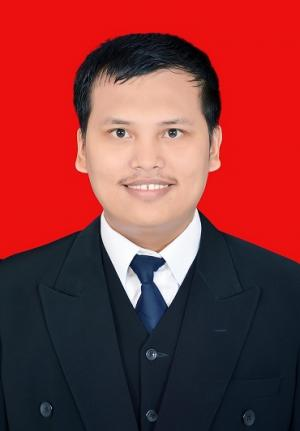
\includegraphics[height = .9\linewidth]{/Person/LukmanMedriavinSilalahi}
\caption{\lr{L. Medriavin Silalahi \cite{silalahi2021improvement}}}
\end{subfigure} 
\begin{subfigure}[b]{.24\linewidth}\centering
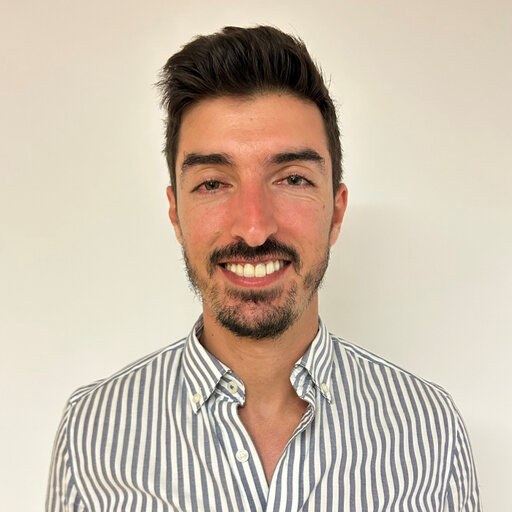
\includegraphics[height=0.9\linewidth]{/Person/MarcoSousa}
\caption{\lr{Marco Sousa \cite{Sousa2021Analysis}}}
\end{subfigure}
\begin{subfigure}[b]{.24\linewidth}\centering
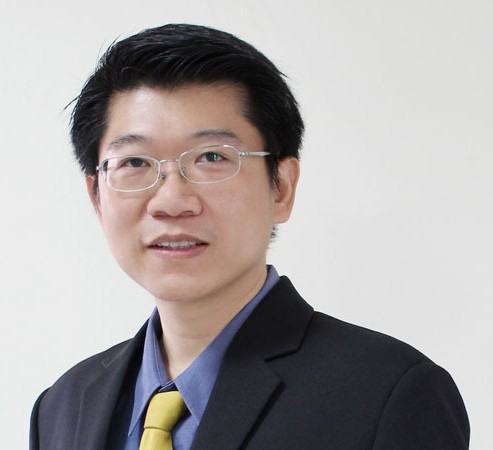
\includegraphics[height=0.9\linewidth]{/Person/peeraponguthansakul}
\caption{\lr{Peerapong Uthansakul \cite{charoenlap2016prediction}}}
\end{subfigure}
\begin{subfigure}[b]{.24\linewidth}\centering
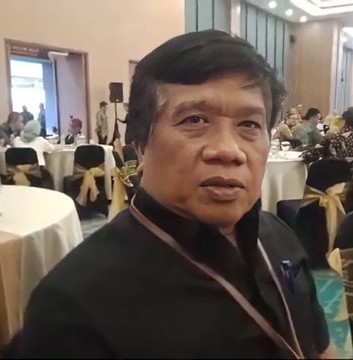
\includegraphics[height=0.9\linewidth]{/Person/YuliarmanSaragih}
\caption{\lr{Yuliarman Saragih \cite{Aprillia2020RF}}}
\end{subfigure}
\end{figure}


\section{حل مشکلات}
\chapter{شرح روش پیشنهادی}
\label{chap:approach}

در این فصل، قصد داریم روشی برای بهینه‌سازی مسیر انجام 
\gls{DriveTest}
ارائه دهیم که با استفاده از آن، دیگر نیازی به بررسی تمامی موقعیت‌ها و نقاط جغرافیایی یک ناحیه از نقشه نیست و می‌توان با پیمایش یک مسیر کوتاه‌تر، به جمع‌آوری داده‌هایی که نشان‌دهنده‌ی وضعیت سیگنال در آن ناحیه هستند، پرداخت. 

در ابتدا، مدل سامانه و فرضیات مساله در 
\autoref{sec:systemmodel}
مورد بررسی قرار می‌گیرد و پس از آن، در 
\autoref{sec:proposedapproach}،
روش پیشنهادی در چهار گام تشریح می‌شود. این رویکرد به گونه‌ای طراحی شده است تا عملگرهای شبکه‌های تلفن همراه بتوانند با بهبود فرآیند جمع‌آوری داده‌ها، کارایی و بهره‌وری عملیات \gls{DriveTest} را افزایش دهند و به‌ طور همزمان هزینه‌ها و زمان مورد نیاز برای انجام این عملیات‌ها را کاهش دهند.

\section{مدل سامانه و فرضیات}
\label{sec:systemmodel}


\begin{table}
	\centering
	\renewcommand{\arraystretch}{2}
	\caption{فهرست نمادها}
	\begin{tabular}{cp{13cm}}
		\toprule
		\textbf{نماد} &  \textbf{توضیحات} \\
		\midrule
		$W\times H$ &
		ابعاد بخش مستطیلی از نقشه \\
		$K$ &
		تعداد ناحیه‌های مستطیلی کوچک \\
		$N$ &
		تعداد کل نقاط بحرانی‌ انتخاب شده برای \gls{DriveTest} \\
		$M$ &
		حداکثر تعداد نقاط بحرانی‌‌ای انتخاب شده در هر ناحیه \\
		$\mathbf{B}^i$ &
		مجموعه‌ی ایستگاه‌های پایه ناحیه $i$-ام \\
		$\mathbf{P}^i$ &
		مجموعه‌ی نقاط بحرانی ناحیه $i$-ام \\
		$\mathbb{C}(i, d_i)$ &
		دایره‌ای به مرکز نقطه‌ی مرکزی ناحیه‌ی $i$-ام و شعاع $d_i$ به اندازه‌ی قطر این ناحیه‌ی مستطیلی \\
		$\mathbf{O}^i$ &
		اجتماع ایستگاه‌های پایه و نقاط بحرانی ناحیه‌ی $i$-ام و ایستگاه‌های پایه و نقاط بحرانی ناحیه‌های همسایه‌ی‌ واقع در دایره‌ی $\mathbb{C}(i, 0.7d_i)$
		\\
		$(\text{lat},\text{lon})$ &
		مختصات نقطه‌ای در دستگاه مختصات جغرافیایی \\
		$\text{lat}_{\min}^i$ &
		حداقل عرض جغرافیایی نقاط ناحیه‌ی $i$-ام \\
		$\text{lon}_{\max}^i$ &
		حداکثر طول جغرافیایی نقاط ناحیه‌ی $i$-ام \\
		\bottomrule 
	\end{tabular}
	\label{tab:symbols}
\end{table}


\section{تشریح روش پیشنهادی}
\label{sec:proposedapproach}
\begin{nttheorem}
	\label{theorem:betweenmeasure}
	در صورتی‌که نسبت جابه‌جایی بین دو اندازه‌گیری متوالی با فاصله یکی از آن‌ها به اندازه کافی کوچک باشد، می‌توان نتیجه گرفت که 
	$d_{i+1} \approx d_i$.
\end{nttheorem}
\begin{proof}
	مثلث مشخص شده در 
%	\autoref{fig:estimateShadowingNoise}
	را یک بار دیگر در نظر بگیرید. از روابط مثلثاتی می‌دانیم که 
	\begin{equation}
		l_{i,i+1}^2 = d_{i+1}^2+d_i^2 - 2d_id_{i+1}\cos\alpha,
		\label{eq:liiid}
	\end{equation}
	که در آن $l_{i,i+1}$ بیانگر میزان جابه‌جایی بین دو اندازه‌گیری متوالی است.
	\\*[1mm]
\end{proof}

اکنون لم زیر را بدین‌منظور در نظر بگیرد.
\begin{lemma}
	\gls{RandomVariable} $\mathrm{P}^d$
	از
	\gls{GaussianDistribution}
	با 
	\gls{Average}  صفر و \gls{StandardDeviation} $\sqrt{2}\sigma$
	پیروی می‌کند. 
\end{lemma}
\begin{lemmaproof}
	می‌دانیم که 
	$n_i\sim\mathcal{N}(0,\sigma)$. 
	و برای نویز

	
	
\end{lemmaproof}


نمایی از الگوریتم پیشنهادی به صورت سودوکد در 
\autoref{alg:tsp}
نشان  داده شده است. 
\begin{algorithm}[t]
	\caption{حل تقریبی مسئله \lr{TSP}}
	\label{alg:tsp}
	\begin{latin}
		\raggedright
		\textbf{Input}: $N$ Critical points, $K$ partitions.\\
		\vspace{2mm}\textbf{Output}: Approximate TSP solution.
		\begin{algorithmic}[1]
			\STATE\vspace{2mm} Initialize $curPart \gets$ bottom-left partition
			\STATE\vspace{2mm} Initialize $curPoint \gets$ a random point in $curPart$
			\STATE\vspace{2mm} Mark $curPoint$ as visited
			\vspace{2mm}\REPEAT
			\vspace{2mm}\WHILE{unvisited points in $curPart$}
			\STATE\vspace{2mm} Find nearest point $nextPoint$ to $curPoint$
			\STATE\vspace{2mm} Mark $nextPoint$ as visited
			\STATE\vspace{2mm} $curPoint \gets nextPoint$
			\vspace{2mm}\ENDWHILE
			\vspace{2mm}\IF{unvisited partitions remain}
			\STATE\vspace{2mm} Move to next partition (spiral/row-by-row)
			\STATE\vspace{2mm} $curPart \gets$ next partition
			\STATE\vspace{2mm} Find nearest point in $curPart$ to $curPoint$
			\STATE\vspace{2mm} $curPoint \gets$ this nearest point
			\STATE\vspace{2mm} Mark $curPoint$ as visited
			\vspace{2mm}\ENDIF
			\vspace{2mm}\UNTIL{all points visited}\vspace{2mm}
		\end{algorithmic}
	\end{latin}
\end{algorithm}


\chapter{شبیه‌سازی}
\label{chap:simulation}

\section{وارد کردن کد در متن}
مثالی از نوشتن کد مطلب درون یک نوشتار:

\begin{latin}
\lstinputlisting[language=Matlab]{Code/code3.m}
\end{latin}

در این مثال یک کد \lr{MATLAB} دیگر وارد می کنیم، با این تفاوت که می خواهیم یکسری از کلمات کلیدی را مشخص کنیم که لاتک آن ها را با رنگی به خصوصی نشان دهد. 
\begin{latin}
\lstset{emph={binornd},emphstyle=\color{Magenta}}
\lstinputlisting[language=Matlab, morekeywords={ksdensity}]{Code/prog3.m}
\end{latin}

مثالی دیگر از نوشتن کد مطلب در یک نوشتار. فقط در این حالت می خواهیم برخی از تنظیمات پیش فرض را که قبل از شروع نوشتار تعیین کرده ایم، تغییر دهیم. 
\begin{latin}
\lstinputlisting[numbers=right,language=Matlab, framexleftmargin=5mm, frame=shadowbox,rulesepcolor=\color{Yellow}]{Code/code4.m}
\end{latin}

در ضمن شما می توانید حتی در خود همین نوشتار اصلی خود کد مورد نظرتان را بنویسید. 
\begin{latin}
\begin{lstlisting}[mathescape=true]
// calculate  $a_{ij}$
$a_{ij} = a_{jj}/a_{ij} + \alpha$;
\end{lstlisting}
\end{latin}
\chapter{نتیجه‌گیری و کا‌ر‌های آینده}
\label{chap:conclusion}

\section{نتیجه‌گیری}


\section{کارهای آینده}

\bibliography{ETC/library.bib}
\printglossary
\printindex

\clearpage
\begin{latin}
\section*{Abstract}


\vskip 5mm
\textbf{Key Words}:

\end{latin}

\newpage
\pagestyle{empty}
\begin{latin}
	\ignorespaces
	\begin{center}
		\begin{table}
			\begin{tabular}{ccc}
				
				
				
				
				& 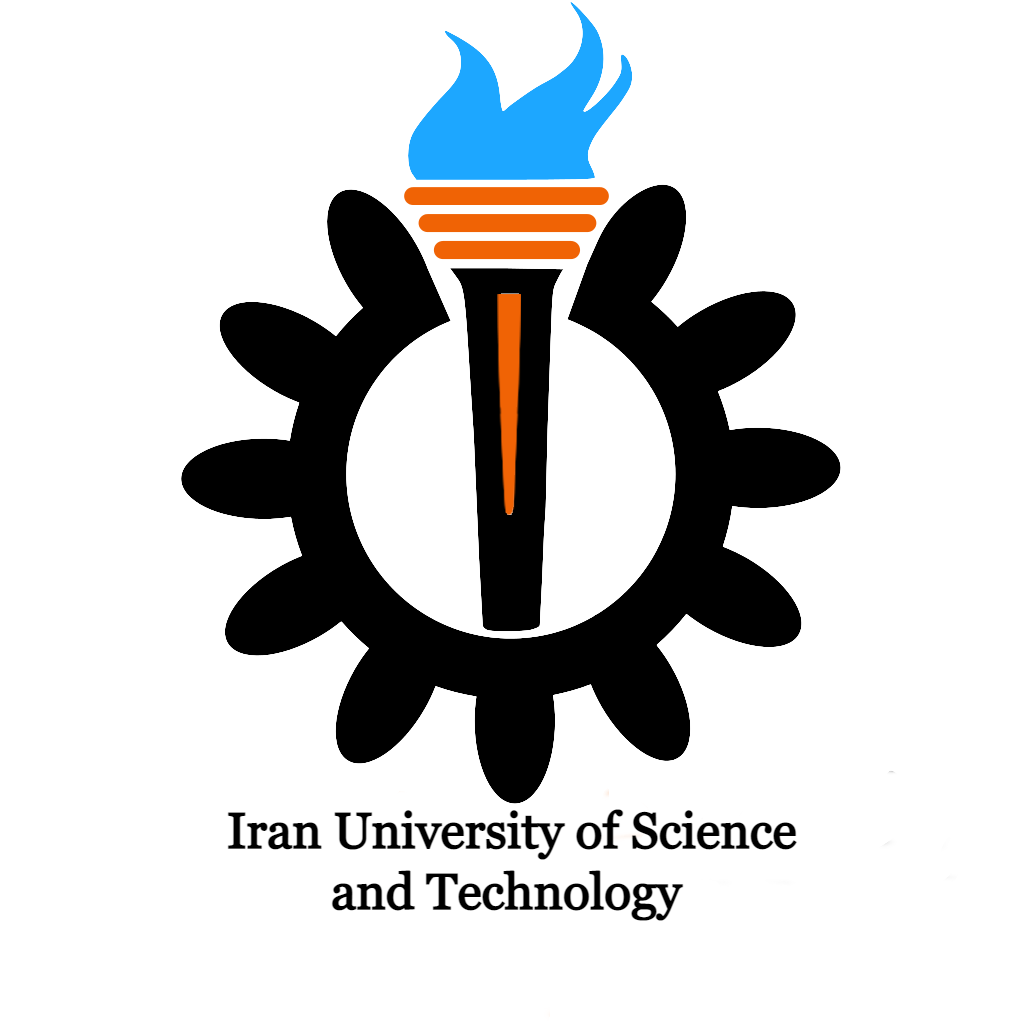
\includegraphics[trim={4cm 3cm 4cm 0.3cm },clip,width=0.24\linewidth]{Logo/En} & \\
				&
				\begin{minipage}{0.55\linewidth}
					\vskip 0.6cm
					\begin{center}
						%\@institute\\* [0.4cm]
						School of Computer Engineering\\ [0.4cm]
						Computer Networks Group \\*[1cm]
					\end{center}
				\end{minipage}
				&
			\end{tabular}
		\end{table}
		\vspace*{\stretch{1}}
		\textbf{{\fontsize{15pt}{50pt}\selectfont\ Title}}
		\vspace*{\stretch{1}}
		\vskip 1cm
		\large{Master's Thesis}\\[.4cm]
		\large{In the field of Computer Engineering—Computer Networks}
		\vspace*{\stretch{1}}
		\vskip 1cm
		\Large{\textbf{Name }}
		\vskip 1.5cm
		\Large{Advisor}
		\\ [0.1cm] \Large{Dr. ......}\\
		%\Large{Co-advisor}
		%	\vskip 0.5cm
		%\\ [0.1cm] \Large{Dr. Abolfazl Diyanat}
		\vskip 2cm
		\large{June 2023}
	\end{center}
	\clearpage
\end{latin}
%%%%%%%%%%%%%%%%%%%%%%%%%%%%%%%%%%%%

\end{document}